%
\begin{floatingfigure}[hr!]{6cm}
 \centering
         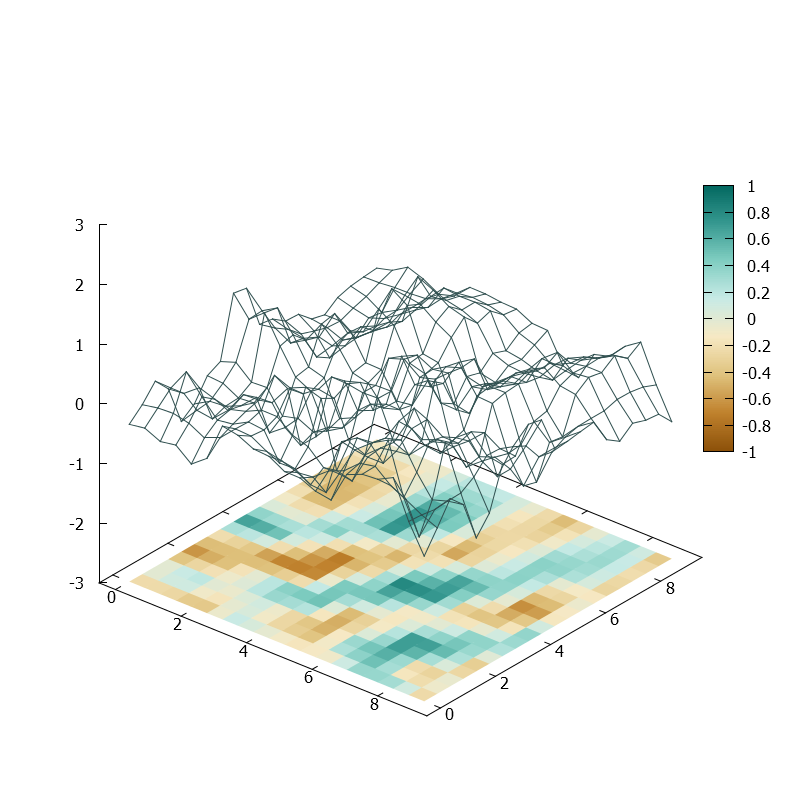
\includegraphics[width=7cm]{img/Plate0_A1.png}
         \caption[Profil einer Phasenmessung]{Normiertes Höhenprofil einer Phasenmessung aus der Sicht von Antenne 1 }
         \label{fig:Plate0_A1_}
\end{floatingfigure}
%
In diesem Abschnitt wird eine Übersicht über die Komplexität des Problems gegeben. In der rechten Abbildung zu sehen ist vergrößert Visualisierung einer Kalibriermessung. Der verwendete Aufbau ist in Abbildung~\ref{fig:Spider1}. gezeigt. Er besteht aus vier Antennen die in einer Ebene angeordnet sind. Es wurde eine reproduzierbare Aufstellung verwendet (Abbildung~\ref{fig:Spider_setup1}) und eine Fläche von $1\times1$ Meter vermessen. Alle $10$ cm wurde eine Messung gespeichert. In der Abbildung kann man deutlich das Verhalten der Phasendaten sehen. Um diesen Verlauf deutlicher zu zeigen wurden die Phasenwerte normiert und als Oberfläche in den Plot gelegt. Am Boden gezeigt ist der Kontur-Plot der Werte. Zwischen den Werten wurde Interpoliert um die Nulldurchgänge deutlicher zu zeigen.\\
%
Die Übersicht aus der Sicht aller Antennen ist in Abbildung~\ref{fig:Real_Measurements} gezeigt.\\
%
In der Abbildung~\ref{fig:Complexity1} werden die Daten ohne Interpolation dargestellt. Es wurden die Höhenlinien eingezeichnet. Die Anordnung der Plots soll ein Gefühl dafür vermitteln, wie die Messwerte eines Tags sich an einer Stelle verhalten.
%
\begin{figure}[h!]
        \centering
        \begin{subfigure}[b]{0.4\textwidth}
            \centering
            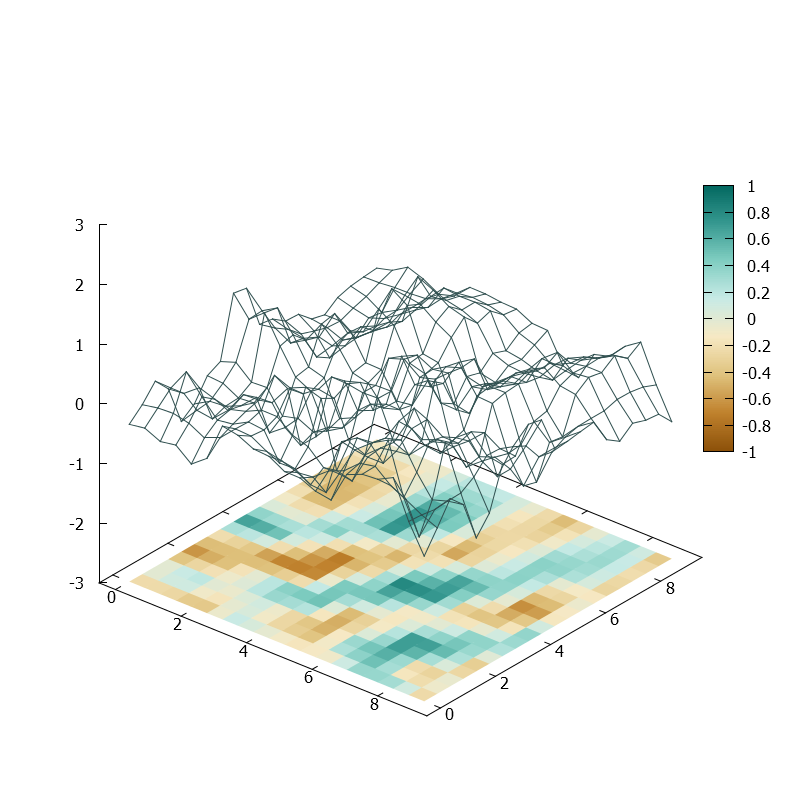
\includegraphics[width=\textwidth]{img/Plate0_A1.png}
            \caption[lorem]{Antenne 1}
            \label{fig:Plate0_A1}
        \end{subfigure}%
\\
        \begin{subfigure}[b]{0.4\textwidth}
            \centering
            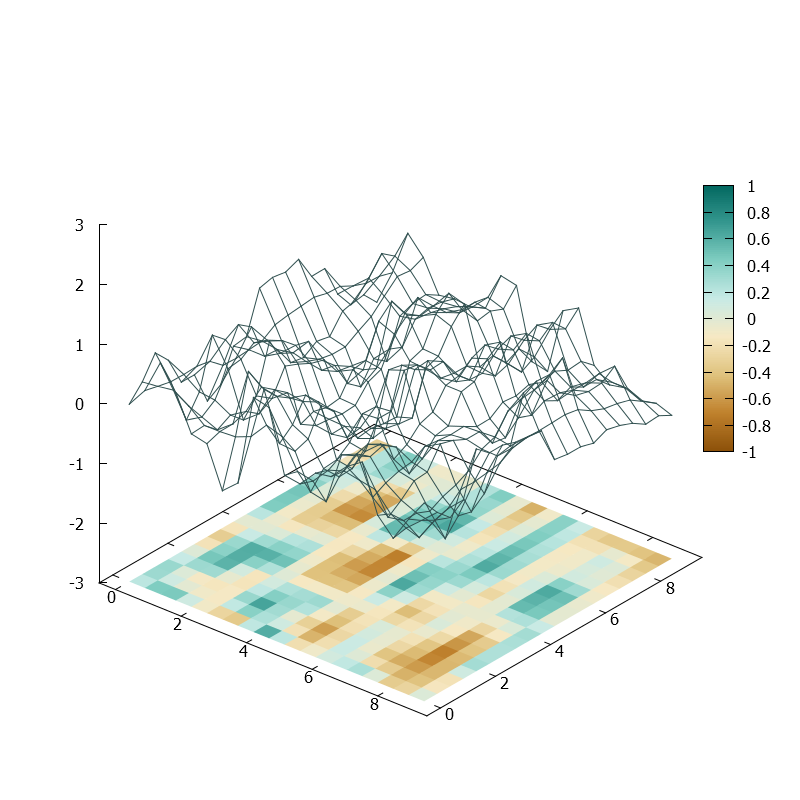
\includegraphics[width=\textwidth]{img/Plate0_A2.png}
          	\caption[Loren ipsum]{Antenne 2}
         	\label{fig:Plate0_A2}
        \end{subfigure}
\qquad\qquad
        %add desired spacing between images, e. g. ~, \quad, \qquad etc.
         %(or a blank line to force the subfigure onto a new line)
        \begin{subfigure}[b]{0.4\textwidth}
			\centering
			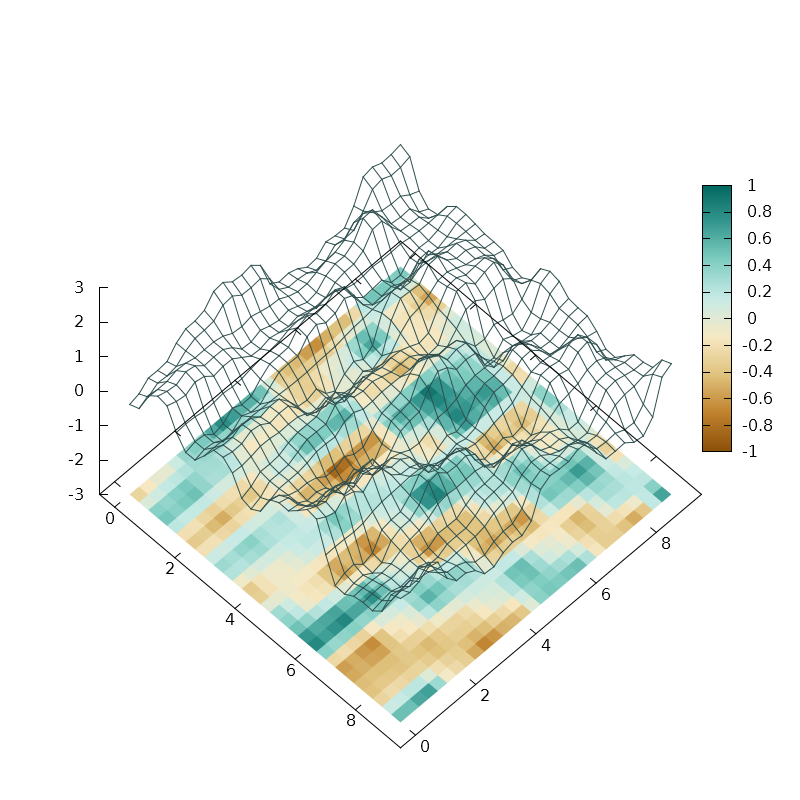
\includegraphics[width=\textwidth]{img/Plate0_A4.png}
			\caption[Loren ipsum]{Antenne 4}
			\label{fig:Plate0_A3}
        \end{subfigure}
\\
        \begin{subfigure}[b]{0.4\textwidth}
			\centering
			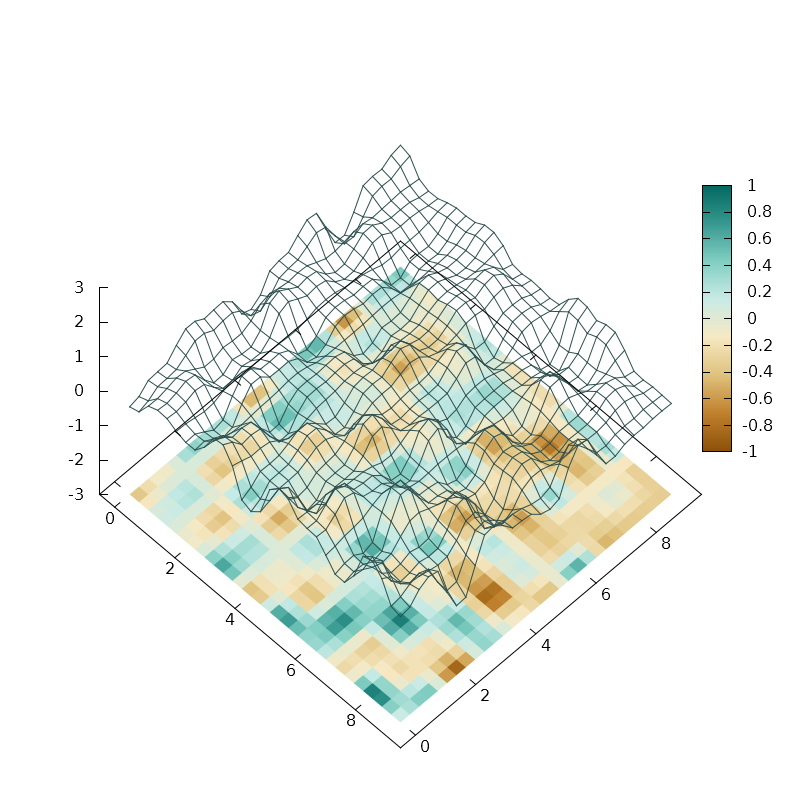
\includegraphics[width=\textwidth]{img/Plate0_A3.png}
			\caption[Loren ipsum]{Antenne 3}
			\label{fig:Plate0_A4}
        \end{subfigure}
        \caption[Reale Messwerte visualisiert]{Blick auf die Messwerte der  Kalibrierplatte aus der "Sicht" der Antennen. Dabei zeigt sich deutlich der Wellencharakter der Messung, dieser ist zu erwarten. Die Messung würden mit bei einer Frequenz von $865,7$ MHz unter Laborbedingungen aufgenommen. }\label{fig:Real_Measurements}
\end{figure}
%
\begin{figure}[ht!]
         \centering
         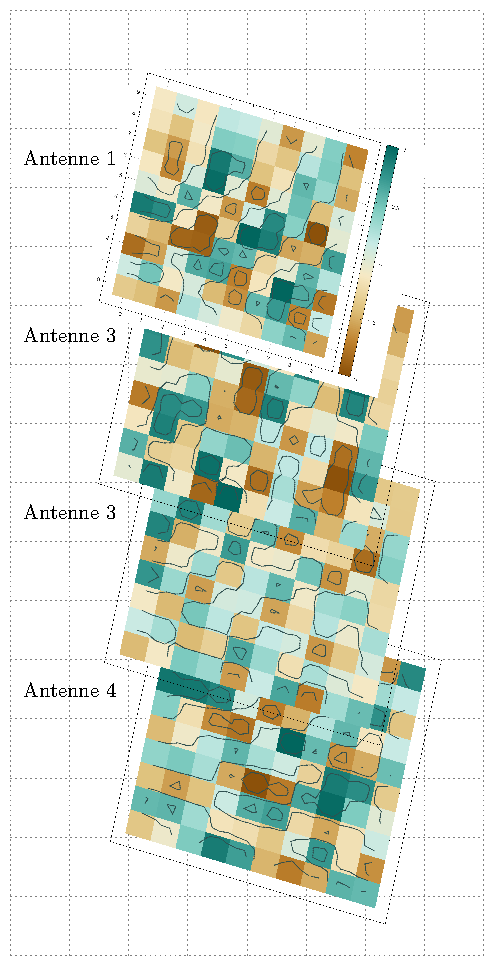
\includegraphics[width=0.6\textwidth]{img/complexitiy1.pdf}
%         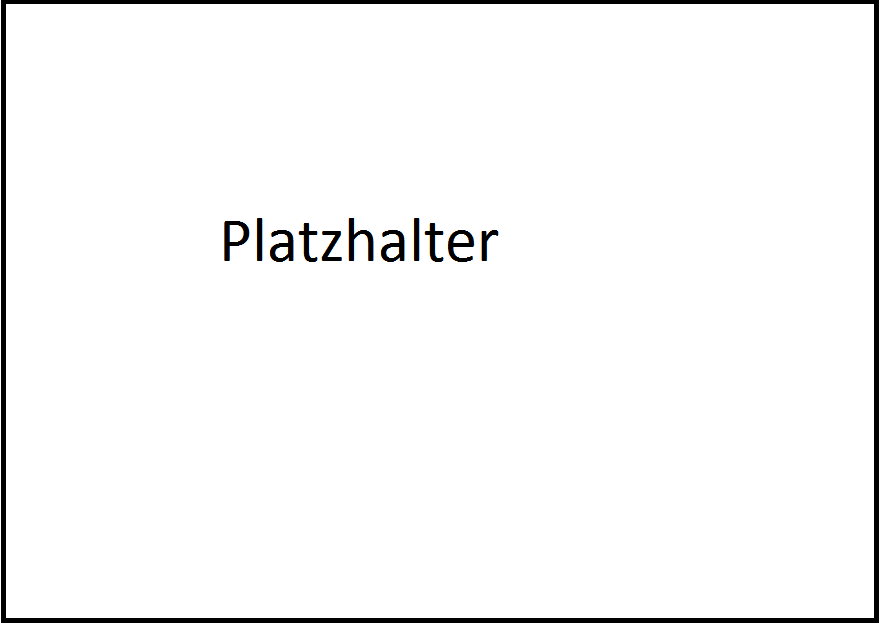
\includegraphics[width=0.7\textwidth]{img/00_placeholder.png}
         \caption[Normierte Messwerte von Kalibriermessung]{Diese Grafik zeigt die Visualisierung von realen Phasen-Messwerten. Die Daten wurden durch Vermessung einer $1\times1$-Kalibrierplatte mit reproduzierbarer Aufstellung gewonnen. Die Daten wurden normiert. In jeder Dimension wurden $10\times10$ Werte aufgenommen. Die Darstellung der Phasenwerte erfolgt als Heatmap, es soll qualitativ der Verlauf der Phasenwerte gezeigt werden. Zur Orientierung sind in jedem Plot Höhenlinien eingezeichnet. Pro Plot werden die Daten einer Antenne dargestellt. Die Antenne von der die Daten stammen ist angegeben.}
         \label{fig:Complexity1}
%
\end{figure}

